\section{Approach}
\label{sec:approach}
% Generalize your work in an abstraction level, e.g., positioning it as a framework rather than a tool
% - What you develop should be beyond your own implementation
% - Then you are in a better position when you discuss limitations of your work
% Try to separate the ideas from (a particular) concrete implementation
% - But sometimes you have to mention it a bit and refer the readers to the implementation section
% Explain some details with examples (even if you have illustrated your high level ideas in the example section)

\begin{figure*}[t]
\centering
%\vspace*{-2ex}
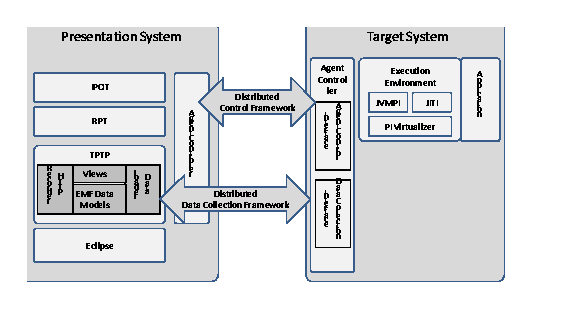
\includegraphics[scale=1.00,clip]{figs/approach.eps}
\caption{The high-level overview} \label{fig:omr}
%\vspace*{-2ex}
\end{figure*}

The high-level overview of our approach is shown in Figure \Fix{prepare for the Figure}.
Our approach consists of two major phases: Correlating Trace Data and Exploiting Statistically Sampled Trace Data.
In the first phase, we focus on correlating (fully-collected) traces from the server side with the client-side performance test data without requiring the involved servers to be ARM-instrumented.
In the second phase, we focus on using statistically sampled traces in the techniques from the first phase instead of full trace data.

\subsection{Correlating Trace Data}
\label{sec:correlating}
In order for performance analyst to navigate from the client-side runtime information to the server-side runtime information in performance analysis, correlating client-side transactions or time-ranges with server-side extrapolated runtime information should be done.
For an ARM-instrumented server, we explore ARM hooks for providing the information on when transactions begin and end. Each ARM instrumented server generates a correlator to map parent transactions to their respective child transactions across multiple processes or servers. Thus, the correlation mechanism can trace the path of a distributed transaction through multiple processes or servers. We further correlate with the runtime information collected via JVM profiling with the information collected via ARM hooks; therefore, we can establish the correlation between the JVM profiling information and the information from the load testing tool at the client side.

Next, we show how to correlate the traces \Fix {add more explanations}
A model generated by RPT is in the format of Eclipse Modeling Framework (EMF\cite{emf}) model. As the traces generated by TPTP are stored as EMF model, the model generated by our approach is also an EMF model.
\\
\\
In case of absence of ARM, we develop learning techniques to discover with transactions begin and end at the server code. There will be three phases in the learning process: training, validation, and analysis.

\subsection{Exploiting Statistically Sampled Trace Data}
\label{sec:statistical}


% IPOT
%This tool identifies the root cause of poor performance observed during a test by round-trip response time %decomposition. The response time is broken down into the times spent within each component in the system under test %enabled by the included Tivoli ARM data collector. An updated Data Collection Infrastructure (DCI) version has been %posted to run with Rational Performance Tester v6.1.2. 